\documentclass[11pt,letterpaper]{article}

\usepackage[utf8x]{inputenc}
\usepackage{ucs}
\usepackage[spanish]{babel}
\usepackage{amsmath}
\usepackage{amsfonts}
\usepackage{amssymb}
\usepackage{graphicx} % Para importar imagenes

\author{Mauricio Mejía Castro}
\title{Solución Taller No. 1 - Análisis de datos con R}

\begin{document}
	\maketitle
	\section{Medidas de tendencia central}
	
	\begin{itemize}
		\item Operador {\em pipeline} ({\tt \%>\%}): Ofrece una sintaxis alternativa a la anidación usual de operaciones {\tt dplyr}. En esencia, permite construir de manera más natural una sucesión de operaciones.
		\item Función {\tt group\_by()}: Operación del paquete {\tt dplyr} que toma una tabla como entrada y retorna una tabla agrupada con respecto a alguna variable.
		\item Función {\tt summarise\_if()}: Este operador ha sido reemplazado por el uso de {\tt across}, según la documentación de R. Su principal uso es el de aplicar una transformación a múltiples columnas de una tabla.
		\item Función {\tt is.numeric()}: Retorna {\tt TRUE} si el tipo de dato es un entero o entero con doble precisión.
	\end{itemize}

	El siguiente código utiliza estas funciones para resumir por medio de la media y la mediana los datos del Apéndice B con respecto a la columna {\tt SamplePosition}.
	
	\begin{verbatim}
		soil_dat_path <- paste(main_path, "appendix-b.csv", sep = "")
		soil_dat <- read.csv(soil_dat_path)
		soil_summary <- soil_dat %>% 
		group_by(SamplePosition) %>% 
		summarise(across(is.numeric, list(Media=mean, Median=median))) 
	\end{verbatim}

	\section{Medidas de dispersión}
	
	El mayor nivel de variación se presenta en los sistemas de producción a campo abierto. Esto lo podemos determinar con el resultado del código adjunto.
	
	\begin{verbatim}
		tomato_summary.1 <- tomato_dat %>% 
		group_by(Department) %>% 
		summarise(across(is.numeric, list(cvar=cv))) 
	\end{verbatim}

	El Cuadro \ref{tab:table-01} resume el cálculo del coeficiente de variación para las variables numéricas agrupadas por la variable {\tt Department}:

	\begin{table}
		\centering
		\begin{tabular}{|c|c|c|c|c|} \hline
			%{\bf class} & {\bf 0} & {\bf 1}\\ \hline
			%V1 & V2 & V3 & V4 & V5\\ 
			Variable & Boyaca & Santander\\ \hline
			Longitude.DD\_cvar & -0.04479261 & -0.06543138\\ 
			Latitude.DD\_cvar & 0.8575635 & 1.7145951\\ 
			Altitude.masl\_cvar &  6.672738 & 15.533085\\ 
			LotArea.m2\_cvar & 44.11184 & 86.60027\\ 
			CycleDuration.days\_cvar & 16.30292 & 10.75022\\ 
			Density.plants.m2\_cvar & 16.64172 & 27.21224\\ 
			Yield.kg.m2\_cvar & 45.67017 & 52.89135\\ 
			IrrigVolumen.l.m2\_cvar &  65.45662 & 141.56878\\ 
			Rainfall.mm\_cvar & NA & 41.19937\\ 
			TotalN.kg.m2\_cvar & 56.79701 & 72.86935\\ 
			P2O5.kg.m2\_cvar & 60.75209 & 85.55578\\ 
			K2O.kg.m2\_cvar & 63.15631 & 76.57278\\   \hline
		\end{tabular}
		\caption{\label{tab:table-01} Coeficientes de variación agrupados por departamento}
	\end{table}
	
	Para conocer a qué instrumento le corresponde el mayor nivel de variación, agrupamos por la variable {\tt DataSource} a través del código adjunto:
	
	\begin{verbatim}
		tomato_summary.2 <- tomato_dat %>% 
		group_by(DataSource) %>% 
		summarise(across(is.numeric, list(cvar=cv))) 
	\end{verbatim}

	El resumen obtenido en el Cuadro \ref{tab:table-02} sugiere que el método de medición con mayor nivel de variación son los seguimientos.

	\begin{table}
		\centering
		\begin{tabular}{|c|c|c|} \hline
			DataSource & FollowUps & Survey\\ \hline
			Longitude.DD\_cvar & -0.2897137 & -0.3014357\\ 
			Latitude.DD\_cvar & 6.276944 & 6.119214\\ 
			Altitude.masl\_cvar & 21.15645 & 18.38336\\ 
			LotArea.m2\_cvar & 100.59032 &  79.97274\\ 
			CycleDuration.days\_cvar & 21.48421 & 25.88937\\ 
			Density.plants.m2\_cvar & 42.57766 & 38.58078\\ 
			Yield.kg.m2\_cvar & 45.50939 & 61.53591\\ 
			IrrigVolumen.l.m2\_cvar & 93.33036 & 83.69995\\ 
			Rainfall.mm\_cvar & 144.8402 & 140.7425\\ 
			TotalN.kg.m2\_cvar & 69.18710 & 73.30321\\ 
			P2O5.kg.m2\_cvar & 87.76013 & 73.37628\\ 
			K2O.kg.m2\_cvar & 84.20972 & 83.40776\\ 
			\hline
		\end{tabular}
		\caption{\label{tab:table-02} Coeficientes de variación agrupados por tipo de medición}
	\end{table}
	
	
	La única variable en la que se evidencia un coeficiente de variación negativo es en la variable {\tt Longitude.DD}. 

	\section{Gráficas para medidas de tendencia central y dispersión}
	La Figura \ref{fig:figure-01} muestra la gráfica generada por el código dado en el enunciado.
	
	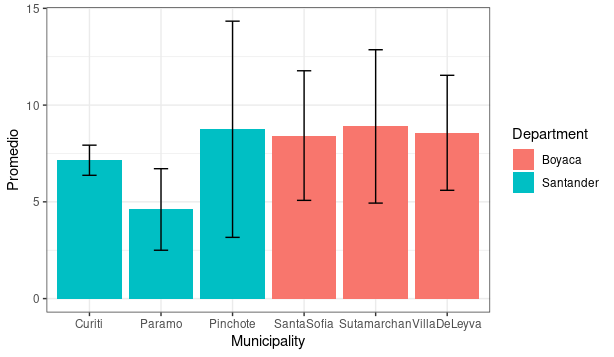
\includegraphics[scale=0.8]{graph_01.png}
	\begin{figure}[h!]
		\caption{\label{fig:figure-01} Comparación del promedio de rendimiento por municipio}
	\end{figure}

	\begin{itemize}
		\item Función {\tt ggplot()}: Inicializa un objeto {\tt ggplot}. Este puede ser usado para empezar el marco inicial sobre el cual puede ser graficado algún conjunto de datos.
		\item Función {\tt aes()}: Proporciona la lista de elementos estéticos que se utilizarán en la gráfica.
		\item Función {\tt theme\_bw()}: Proporciona temas visuales completos para la gráfica.
		\item Función {\tt geom\_bar()}: Indica al objeto que la gráfica debe ser de barras.
		\item Función {\tt geom\_errorbar()}: Agrega un gráfico de intervalo vertical a la gráfica de barras.
	\end{itemize}

	\section{Medidas de posición relativa}
	En la Gráfica \ref{fig:figure-02} se muestra el resultado del código dado.
	
	Si nos detenemos en el nivel de acidez ({\tt pH}), es válido mencionar que existe mayor dispersión de esta para los sistemas bajo invernadero (Boyacá) que para los de campo abierto (Santander). Se evidencian más valores atípicos en sistemas de campo abierto que en los de bajo invernadero. Se observa también que en ambos sistemas, el nivel de acidez exhibe asimetría negativa.
	
	\vspace{1cm}
	
	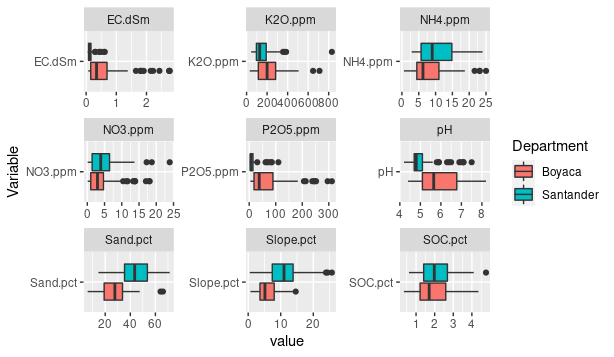
\includegraphics[scale=0.8]{graph_02.png}
	\begin{figure}[h!]
		\caption{\label{fig:figure-02} Comportamiento de algunas variables en el conjunto de datos}
	\end{figure}
	
\end{document}